\documentclass[a4paper,11pt]{article}
\usepackage[T1]{fontenc}
\usepackage[utf8]{inputenc}
\usepackage{lmodern}
\usepackage{graphicx}

\title{B-Tag 2015}
\author{Thomas, Josua, Niclas, Andreas}

\begin{document}

\maketitle
\tableofcontents

\section{Aufgaben}
\subsection{Aufgabe 1: Dreiecksgeometrie}
Diagramm:

\begin{figure}[htbp] 
        \centering
        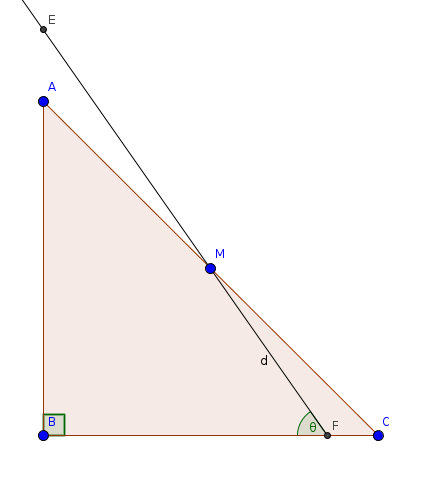
\includegraphics[width=6cm]{img/A1_1.png}
\end{figure}

Wir wollen eine Funktion $\overline{FE}(\theta)$ aufstellen, und zeigen, dass diese immer gr\"o\ss er als CA ist.

1. Wie lang ist die Strecke $\overline{FM}$?
\[ \overline{FM}(\theta) = \frac{M_y}{sin(\theta)} \]

2. Wie lang ist die Strecke $\overline{ME}$?
\[ \overline{ME}(\theta) = \frac{M_x}{sin((\pi/2)-\theta)} \]

3. Die Strecke $\overline{FE}$ ist also $\overline{FM} + \overline{ME}$ (natürlich alles im Definitionsbereich $0 < \theta < \frac{\pi}{2}$:
\[ \overline{FE}(\theta) = \frac{M_y}{\sin(\theta)} + \frac{M_x}{\sin((\pi/2)-\theta)} \]

Jetzt muss gezeigt werden, dass der Tiefpunkt von $\overline{FE}(\theta)$ den Wert $\overline{AC}$ hat. Dazu wird $\overline{FE}(\theta)$ zuerst abgeleitet, um den TP zu finden:

%\[ \overline{FE}'(\theta) = - \frac{M_y \cos(\theta)}{(\sin(\theta))^2} + \frac{M_x \cos(\theta - (\pi/2))}{\sin((\pi/2)-\theta)^2} \]
\[ \overline{FE}'(\theta) = \frac{M_x (\sin(\theta))^3 - M_y (\cos(\theta))^3)}{(\sin(\theta))^2 (\cos(\theta))^2} \]

Jetzt setzen wir $\overline{FE}' = 0$, um den Tiefpunkt von $\overline{FE}(\theta)$ bei $\theta = \frac{\pi}{4}$ zu finden, und sehen, dass $FE(\frac{\pi}{4}) = CA$ ist. Daher ist $\overline{FE}$ immer länger als $\overline{CA}$ (au\ss er bei $\theta=\frac{\pi}{2}$).

\subsection{Aufgabe 2: Verschiebungen}

\subsection{Aufgabe 3: St\"ocke}

\end{document}
